\def\mterm#1{{\upshape \bfseries #1}}
\def\mra{x_1,\dots,x_k}
\def\prim{\textsc{prim}\xspace}
\def\URM{\textsc{urm}\xspace}
\def\renderURM#1{$$\directlua{
   urm=require("urm.lua")
   urm.RenderFromTable({#1})}$$
}

\chapter{Computability Theory}

\epigraph{Finally, we express our immense gratitude to Gwyn Mitchell, who typed 
the master copy from which this book is reproduced. If ever there is an Award 
for Layout of Commutative Diagrams, we feel sure that it will be hers. 
}{---Michael A. Arbin and Ernest G. Manes in \textit{Arrows, structures, and functors: the categorical imperative.}}

\section{What is Computability}

We begin this chapter with a discussion of the fundamental idea of an 
algorithm or effective procedure. In subsequent sections we describe the 
way in which this idea can be made precise using a kind of idealised 
computer; this lays the foundation for a mathematical theory of computability and computable functions.
 
\subsection*{Algorithms, or effective procedures}
 
When taught arithmetic in junior school we all learnt to add and 
to multiply two numbers. We were not merely taught that any two 
numbers have a sum and a product - we were given methods or rules for 
finding sums and products. Such methods or rules are examples of 
algorithms or effective procedures. Their implementation requires no 
ingenuity or even intelligence beyond that needed to obey the teacher's 
instructions. 

More generally, an algorithm or effective procedure is a mechanical 
rule, or automatic method, or programme for performing some  
mathematical operation. Some more examples of operations for which easy 
algorithms can be given are 

(1.1) (a) given n, finding the nth prime number, 

(b) differentiating a polynomial, 

(c) finding the highest common factor of two numbers (the 
Euclidean algorithm), 

(d) given two numbers $x$, $y$ deciding whether $x$ is a multiple of $y$. 


When an algorithm or effective procedure is used to calculate the 
values of a numerical function then the function in question is described 
by phrases such as \emph{effectively calculable}, or \emph{algorithmically computable}, or 
effectively computable, or just computable. For instance, the functions $xy$, 
$HCF(x, y) =$ the highest common factor of $x$ and y, and /(n) = the nth 
prime number, are computable in this informal sense, as already 
indicated. Consider, on the other hand, the following function: 
\[
g(n) = \begin{cases}
1\quad \parbox{0.7\textwidth}{ if there is a run of exactly n consecutive 7s in the decimal expansion of $\pi$},\\
0\quad \text{ otherwise.}
\end{cases}
\]
 
 
Most mathematicians would accept that g is a perfectly legitimate 
function. But is $g$ computable? There is a mechanical procedure for 
generating successive digits in the decimal expansion of $\pi$, so the 
following ``procedure'' for computing $g$ suggests itself. 
 
'Given $n$, start generating the decimal expansion of tt, one digit at a 
time, and watch for 7s. If at some stage a run of exactly n consecutive 7s 
has appeared, then stop the process and put g(n ) = 1. If no such sequence 
of 7s appears put g(n) = 0.' 

The problem with this 'procedure' is that, if for a particular n there is no 
sequence of exactly n consecutive 7s, then there is no stage in the process 
where we can stop and conclude that this is the case. For all we know at 
any particular stage, such a sequence of 7s could appear in the part of the 
expansion of tt that has not yet been examined. Thus the 'procedure' will 
go on for ever for inputs n such that g(n) = 0; so it is not an effective 
procedure. (It is conceivable that there is an effective procedure for 
computing g based, perhaps, on some theoretical properties of tt. At the 
present time, however, no such procedure is known.) 

This example pinpoints two features implicit in the idea of an effective 
procedure - namely, that such a procedure is carried out in a sequence of 
stages or steps (each completed in a finite time), and that any output 
should emerge after a finite number of steps. 

So far we have described informally the idea of an algorithm, or 
effective procedure, and the associated notion of computable function. 
These ideas must be made precise before they can become the basis for a 
mathematical theory of computability - and non-computability. 

\subsection*{URM}

Our first mathematical idealisation of a computer is called an 
unlimited register machine (\URM); it is a slight variation of a machine 
first conceived by Shepherdson \& Sturgis\footcite{shepherdson1963}. In this section we 
describe the \URM and how it works; we begin to explore what it can do in 
§3. We have to stress that this is a simple machine. For notions of what a machine is see
Minsky\footcite{minsky1967}. These machines are modeled after real computers and are often called
Random Access Machines (RAM). 

A \URM has an array of \emph{registers} $R_1, R_2, R_3,\dots$ which store natural numbers $r_1,r_2,\dots$

\[
\begin{array}{|c|c|c|c|c|c|c|c}
\hline
R_1 & R_2 &R_3 &R_4 &R_5 &R_6 &R_7 &\dots\\
\hline
r_1 & r2  &r3  &r4  &r5  &r6  &r7  &\dots\\
\hline
\end{array}
\]

The contents of the registers may be altered by the \URM in response to 
certain instructions that it can recognise. These instructions correspond to 
very simple operations used in performing calculations with numbers. A 
finite list of instructions constitutes a \emph{program}. The instructions are of four 
kinds, as follows.\footnote{We follow Nigel Cutland's description} 


\paragraph{Zero instructions} For each $n = 1, 2, 3,\dots$ there is a zero instruction 
$Z(n)$. The response of the \URM to the instruction $Z(n)$ is to change the 
contents of $R_n$ to 0, leaving all other registers unaltered. 

Suppose that the \URM is in the following 
configuration 
\[
\begin{array}{|c|c|c|c|c|c|c|c}
\hline
R_1 & R_2 &R_3 &R_4 &R_5 &R_6 &R_7 &\dots\\
\hline
9 & 6  &5  &  &23  &7  &0  &\dots\\
\hline
\end{array}
\]
and obeys the zero instruction Z(3). Then the resulting configuration is
\[
\begin{array}{|c|c|c|c|c|c|c|c}
\hline
R_1 & R_2 &R_3 &R_4 &R_5 &R_6 &R_7 &\dots\\
\hline
9 & 6  &5  &  &23  &7  &0  &\dots\\
\hline
\end{array}
\]

The response of the \URM to a zero instruction $Z(n)$ is denoted by $0\rightarrow R_n$ or $r_n :=0$ the latter reads as $r_n$ becomes 0.


\paragraph{Successor instructions} For each $n = 1,2,3,\dots$ there is a successor 
instruction $S(n)$. The response of the \URM to the instruction S(n) is to 
increase the number contained in $R_n$ by 1, leaving all other registers 
unaltered. 

Example Suppose that the \URM is in the configuration (*) 
above and obeys the successor instruction \S(5). Then the new  
configuration is 
\[(*)
\begin{array}{|c|c|c|c|c|c|c|c}
\hline
R_1 & R_2 &R_3 &R_4 &R_5 &R_6 &R_7 &\dots\\
\hline
9 & 6  &5  &  &23  &7  &0  &\dots\\
\hline
\end{array}
\]
The effect of a successor instruction $S(n)$ is denoted by $r_n+1\rightarrow R_n$ or 
$r_n := r_n+1$ ($r_n$ becomes $r_n +1$). 

\paragraph{Transfer instructions.} For each $m = 1, 2, 3,\dots$ and $n = 1, 2, 3,\dots$ there 
is a transfer instruction $T(m,n)$. The response of the \URM to the 
instruction $T(m, n)$ is to replace the contents of $R_n$ by the number $r_m$ 
contained in $R_m$ (i.e. transfer $r_m$ into $R_n$); all other registers (including 
$R_m$) are unaltered. 

Example Suppose that the \URM is in the configuration (**) 
above and obeys the transfer instruction ${\rm T}(5,1)$. Then the resulting 
\begin{equation}
\begin{array}{|c|c|c|c|c|c|c|c}
\hline
R_1 & R_2 &R_3 &R_4 &R_5 &R_6 &R_7 &\dots\\
\hline
9 & 6  &5  &  &23  &7  &0  &\dots\\
\hline
\end{array}
\end{equation}
The response of the \URM to a transfer instruction $T(m, n)$ is denoted by 
$r_m\rightarrow R_n$, or $r_n := r_m$ ($r_n$ becomes $r_m$).

 
Let us consider the computation by the \URM under this program with 
initial configuration 
\begin{equation}
\begin{array}{|c|c|c|c|c|c|c|c}
\hline
R_1 & R_2 &R_3 &R_4 &R_5 &R_6 &R_7 &\dots\\
\hline
9 & 6  &5  &  &23  &7  &0  &\dots\\
\hline
\end{array}
\end{equation}
(We are not concerned at the moment about what function this program 
actually computes; we wish to illustrate the way in which the \URM 
operates programs in a purely mechanical fashion without needing to 
understand the algorithm that is being carried out.) 
We can represent the progress of the computation by writing down the 
successive configurations that occur, together with the next instruction to 
be obeyed at the completion of each stage. 
 
 
\paragraph{Jump instructions} In the operation of an informal algorithm there may 
be a stage when alternative courses of action are prescribed, depending 
on the progress of the operation up to that stage. In other situations it may 
be necessary to repeat a given routine several times. The \URM is able to 
reflect such procedures as these using jump instructions; these will allow 
jumps backwards or forwards in the list of instructions. We shall, for 
example, be able to use a jump instruction to produce the following 
response: 

\begin{quote}
If $r2 = r6$, go to the 10$^{\text{th}}$ instruction in the program; otherwise, go 
on to the next instruction in the program.\footnote{This is the common |goto| in programming. In languages like basic the goto used the number of the line. Modern languages use labels and normally frown upon the usage of a |goto| statement.}
\end{quote}


The instruction eliciting this response will be written $\mathrm{J}(2,6,10)$. 

\subsection*{Computations}
To perform a computation the \URM must be provided 
with a program P and an initial configuration - i.e. a sequence 
$a_1, a_2, a_3,\dots$ of natural numbers in the registers $R_1, R_2, R_3,\dots$ 
Suppose that $P$ consists of s instructions $I I2,..., Is$ The \URM begins 
the computation by obeying $I_1$ then $I_2$, $I_n$, and so on unless a jump 
instruction, say $J(m, n, q)$, is encountered. In this case the \URM proceeds 
to the instruction prescribed by $J(m, n, q)$ and the current contents of the 
registers $Rm$ and $R$. We illustrate this with an example.

Consider the following example:

\[
\begin{array}{ll}
I_1 &J(l,2,6) \\
I_2 &S(2) \\
I_3 &S(3) \\
I_4 &J(l,2,6)\\ 
I_5 &J(l,l,2) \\
I_6 &T(3,l) 
\end{array}
\]

We consider the computation by the \URM under this program with an initial configuration


\begin{Example}
As an example we will show how to add two numbers $(x+y)$ together. We cna obtain x+y by adding 1 to x (using the successor instruction) y times. A program 
\end{Example}

\renderURM{"x+k","y","k",0,0,"..."}


The program will be designed to stop when $k=y$ leaving $x+y$ in $R_1$ as required.

The procedure we wish to employ in our program is as follows:
\[
\begin{array}{ll}
I_1 &J(3,2,5) \\
I_2 &S(1) \\
I_3 &S(3) \\
I_4 &J(1,1,1)\\ 
\end{array}
\]
The instruction $I_4$ has the effect of always jumping back to the first instruction. The program will stop by a jump to $I_5$ which does not exist and which according to the \URM rules it will then result in a \textsc{stop} instruction. Thus the $x+y$ is computable. 

It is easy to see that the program $P$ in the Example, given any input  $(n,m)$, gives output $n+m$, that is the program carries out \emph{addition}.

\begin{tcolorbox}[colback=white]
Input convention: To input a k-tuple ($n_1,\dots, n_k$), we start with $n_1,\dots, n_k$
in registers $R_1,\dots,R_k$, respectively, and with $0$ in all the other registers.

Output convention: If a computation halts, the output is the number in
register $R_1$ — there is no output otherwise.
\end{tcolorbox}



\section{Typesetting}

I did not want to interrupt the write up until we came to this point. In order to typeset nicely
the \URM diagrams we will need a number of helper macros.

\subsection*{URM diagram}
Our first concern is to develop a method to typeset the \URM diagrams without much effort. These are
typeset using an array environment and if we need them numbered we can enclose them in an |equation|  environment.

\begin{texexample}{URM}{ex:urm0}
\begin{equation}
\begin{array}{|c|c|c|c|c|c|c|c}
\hline
R_1 & R_2 &R_3 &R_4 &R_5 &R_6 &R_7 &\dots\\
\hline
9 & 6  &5  &  &23  &7  &0  &\dots\\
\hline
\end{array}
\end{equation}
\end{texexample}

As it will be nicer to have a macro of the form \cs{renderURM}\meta{values}. We will use Lua to develop
it. This could also be developed using \latex alone, but we can get fancier using Lua.

\begin{texexample}{URM}{ex:urm1}
\begin{luacode}
local urm = require("urm.lua")
tex.print("\\[")
urm.RenderFromTable({1,2,3,4,5,6,7})
tex.print("\\]")
\end{luacode}
\end{texexample}




\renderURM{1,2,3,4,5,6,7}


Ideally we would like to develop also routines to store, print and execute a program so we can typeset its execution. Since Lua can store functions in a table this might not be that difficult. 



\section{Computability or Recursion Theory}

One of the better books on Computability Theory is Cooper\footcite{cooper2004}. The textbook is at the undergraduate level and explains well many of the fundamentals. An earlier book by Nigel Cutland, \textit{An Introduction to Recursive Functions} is more appealing to the Computer Science student, as it gives parallels and short flow diagrams explaining some of the maths in a more familiar notation. Both books are excellent introductions. If you are new to the topic, my suggestion have a quick glance at both books and then start from Cutland and then Cooper. If you are a student you are at the mercy of your lecturer and his textbook. Whatever you do, the most important point is to understand the reasoning behind the theory.  
\marginpar{\includegraphics[width=0.9\linewidth]{dedekind}}



First we note that some particularly simple functions are 
computable; from these basic functions (defined below) we 
shall then build more complicated computable functions using the  
techniques developed in subsequent sections. 
\bigskip

\begin{Definition}[The Primitive Recursive Functions]
\mbox{}
\vspace*{-10pt}
\begin{enumerate}
\item The initial functions (a) - (c) are primitive recursive:

\begin{enumerate}
\item The \mterm{zero function} is defined by
      \[0(n)=0, \quad \forall n \in \mathbb{N}\]
\item The \mterm{successor function} defined by
      \[n' = n +1,\quad \forall n \in \mathbb N\]
\item The \mterm{projection function} $U^k_i$ is defined by
     \[U_i^k(\mra) = m_i, \text{ each } k\ge1, \text{ and } i=1,\dots,k, \]      
\end{enumerate}
\item If $g,h,h_0,\dots,h_1$ are primitive recursive, then so is $f$ obtained from  $g,h,h_0,\dots,h_1$ by one of the rules:
\begin{enumerate}
 \item {\upshape \textbf{Substitution}}, given by:
     \[f(\mra) = g(h_0(\mra),\dots,h_l(m))\]
     
 \item \mterm{Primitive recursion}, given by:
      \begin{subequations}
       \begin{align}    
         f(m,0)   &= g(m),\\
         f(m,n+1) &=h(m,n,f(m,n)).
       \end{align}
    \end{subequations}   

       
\end{enumerate} 
\end{enumerate}
\end{Definition}

We write \prim for all primitive recursive functions.

For the computer scientist \emph{recursion} is a familiar programming technique, which has a computational role going back to the nineteenth century. 




\section{Programs and Programming} 

Further study here could include 
topics such as the generation of programming languages and the structure 
of programs; and the semantics of programming languages (which we 
touched upon in chapter 10). Texts which cover these matters include 
Arbib [1969], Bird [1976], Brainerd \& Landweber [1974], Engeler 
[1973] and Manna [1974]. 



\section{Notations, basic terminology}

In this first section we want to informally define the basic terminology that is
used throughout the whole book. We use the usual notations
\begin{eqnarray*}
\mathbb{N} &=& \setof{0, 1, 2, \ldots}\text{ for the natural numbers} \\
\mathbb{Z} &=& \setof{\ldots, -2, -1, 0, 1, 2, \ldots}\text{ for the integer
numbers} \\
\mathbb{Q} &=& \setof{\frac{a}{b} \mid a,b \in \mathbb{Z},\ b \neq 0}\text{
for the rational numbers}
\end{eqnarray*}

For the operations on sets we use $\cup$ for the union and $\cap$ for the
intersection. Also $A \subset B$, $a \in A$, $a \not\in A$, $\bar{A}$, $A
\setminus B$, $A \times B$ and $\emptyset$ have their usual meaning.

For the power set of a set $A$ we write $\powset{A}$. $\card{A}$ denotes
the cardinality of $A$.

Logical implication is denoted by $\Rightarrow$.

{\bf Mappings} are denoted by $f : A \to B$ in which case $f$ is a
total mapping. We write $Q(f) = A,\ Z(f) = B$.\footnote{The letters $Q, Z$ stem 
from the German words ''Quelle'' (source) and ''Ziel'' (target).}

If $f: A \to B,\ g : B \to C$ are mappings, then $f \circ g : A
\to C$ is the {\bf composition} which one gets by applying $f$ first and then 
$g$:
\[(f \circ g)(a) = g(f(a))\]

If $f:A \to B$ and $C \subset A$, then $f(C) = \setof{f(c) \mid c \in C }$.

A subset $R \subset A \times B$ is called a {\bf relation} between $A$ and $B$.
\[R_f = \setof{(a,b) \mid b = f(a) } \subset A \times B\] 
is the relation {\bf induced by} the mapping f or also the {\bf graph} of $f$.

Let $f : A \to B$ be a mapping, $A_1 \subset A$ and $g : A_1 \to
B$ a mapping. $f$ is called the {\bf continuation} of $g$ if $f(a_1) = g(a_1),\ 
a_1 \in A_1$. In this case we also write $f \mid _{A_1} = g$, in words: $f$ {\bf
restricted to} $A_1$.

A {\bf semi-group} consists of a set $M$ and an associative operation on that
set, usually written as a multiplication. If a semi-group is commutative, we
also use ''$+$'' instead of ''$\cdot$''.

\index{monoid}
A semi-group is a {\bf monoid} if $M$ contains a neutral element. We often
denote the neutral element with $1_M$ or shortly $1$. In the commutative case we
often write $0$ instead of $1$.

For $A,B \subset M$ the set
\[ A \cdot B = \setof{a \cdot b \mid a \in A,\ b \in B} \]
is the {\bf complex product} of $A$ and $B$.

A subset $A \subset M$ is a {\bf submonoid} of $M$, if $1_M \in A$ and $A$ is
closed under the operation of $M$.

For an arbitrary subset $A \subset M$, the set $A^*$ is the smallest submonoid
of $M$ containing $A$.

More specific:
\[ A^* = \bigcap_{S \in M(A)} S	\]
where 
\[ M(A) = \setof{S \mid S\text{ is a submonoid of }M, A \subset S} \]

It is easy to see that
\[ A^* = \bigcup_{n \geq 0} A^n\text{ with }A^0 = \setof{1}\text{ and } A^{n+1}=
A^n \cdot A \]

In the same sense $A^+ = A^* \setminus \setof{1}$ is defined for semi-groups.

$A$ is called a {\bf generating system} of $A^*$ resp.\ $A^+$.

A special meaning for us has the set of {\bf words} ({\bf strings}) over
a fixed set (alphabet) )$A$. We define words as the finite sequences
of elements of $A$, for example sequences like $(a,b,d,a,c)$ over the alphabet
$A = \setof{a,b,c,d }$.

We define
\[ \mathrm{WORD}(A) := \setof{\epsilon} \cup A \cup (A \times A) \cup (A \times
A \times A) \cup \ldots \]
as the {\bf set of words (strings) over} $A$. 

The symbol $\epsilon$ denotes the {\bf empty word} over $A$, i.e.\ $A^0 =
\setof{\epsilon}$.

If $v, w \in \mathrm{WORD}(A)$, then $v \cdot w$ is the word which you get by
concatenating $v$ and $w$, formally:
\[ v = (a_1, \ldots, a_k),\ w = (a_{k+1}, \ldots, a_n) \Rightarrow v \cdot
w := (a_1, \ldots, a_n) \]

With this operation $\mathrm{WORD}(A)$ becomes a monoid which usually is also
named $A^*$.

This naming is slightly inconsistent because for the first definition of
the ${}^*$-operator it holds $(A^*)^* = A^*$ but for the second usage of the
${}^*$-operator it holds $(A^*)^* \neq A^*$.

\medskip
The following example should clarify this:

Let $A = \setof{a,b,c}$ and $(a,b,a),\ (b,a) \in A^*$.
\begin{eqnarray*}
& (a,b,a)\cdot(b,a) = (a,b,a,b,a) \in A^* \\
& ((a,b,a),(b,a)) \in (A^*)^*\text{, but }\notin A^*
\end{eqnarray*}

Instead of $(a)$ we just write $a$. In this sense it holds $A \subset A^*$. This
also holds in the sense of the first definition of $A^*$.

If $w = (w_1, \ldots, w_n)$, we set $|w| := n$ and call it the {\bf length} of
$w$. Obviously $|w \cdot v| = |w| + |v|$ and $|\epsilon| = 0$.

(Later in this book, the notation $|w|$ is mainly used for reduced words and
the string length is then denoted by $\len{w}$.)

The {\bf reverse} or {\bf mirror} of a word $w = (w_1, \ldots, w_n)$ is the word
$w^R = (w_n, \ldots, w_1)$ and $\epsilon^R = \epsilon$. It holds:
\[ (w \cdot v)^R = v^R \cdot w^R \]

In $A^*$ the {\bf cancellation rules} hold:
\begin{enumerate}
  \item $w \cdot x = w \cdot y \Rightarrow x = y$
  \item $x \cdot w = y \cdot w \Rightarrow x = y$
\end{enumerate}

We define {\bf left} and {\bf right quotient}:
\[ \inv{X} \cdot Y = \setof{w \mid \exists x \in X,\ y \in Y\text{ with }x
\cdot w = y } \]
and 
\[ X \cdot \inv{Y} = \setof{w \mid \exists x \in X,\ y \in Y\text{ with } w
\cdot y = x } \]

Because of the cancellation rules it holds: $\inv{\setof{w}} \cdot \setof{v}$
and $\inv{\setof{w}} \cdot \setof{v}$ are either empty or contain a single
element.

If $\inv{\setof{w}} \cdot \setof{v}$ is not empty, we call $w$ a {\bf
prefix} of $v$.

if $\setof{w} \cdot \inv{\setof{v}} \neq \emptyset$, we call $v$ a {\bf suffix}
of $w$.

In the future we will sometimes just write $w$ instead of $\setof{w}$ and
$w$ {\bf is prefix of} $v$, if $\inv{w} \cdot v \neq \emptyset$.

\bigskip
\begin{exercise}
Let $X$ be an alphabet, $R \subset X^* \times X^*$ a relation on $X^*$. $R$ is
called
\begin{itemize}
  \item {\bf reflexive}: $\Leftrightarrow$ for all $x \in X^*$ it holds $(x, x)
  \in R$
  \item {\bf symmetric}: $\Leftrightarrow$ for all $x, y \in X^*$ it holds $(x,
  y) \in R \Rightarrow (y, x) \in R$
  \item {\bf transitive}: $\Leftrightarrow$ for all $x, y, z \in X^*$ it holds
  $(x, y) \in R,\ (y, z) \in R \Rightarrow (x, z) \in R$
\end{itemize}

Given a relation $R$, construct a relation $R'$ such that
\begin{enumerate}
  \item $R \subset R'$
  \item $R'$ is reflexive, symmetric and transitive
  \item $R' \subset R''$ for all relations $R''$ that fulfill 1) and 2).
\end{enumerate}

$R'$ is called the {\bf equivalence relation} generated by $R$. 
\end{exercise}


\pgfdeclarelayer{edgelayer}
\pgfdeclarelayer{nodelayer}
\pgfsetlayers{edgelayer,nodelayer,main}
\tikzstyle{none}=[inner sep=0pt]
\tikzstyle{box}=[rectangle,fill=white,draw=black]
\tikzstyle{triangle_down}=[regular polygon,regular polygon sides=3,shape border
rotate=180,fill=white,draw=black]

\tikzstyle{filled_vertex}=[circle,fill=black!50,minimum size=2pt,inner sep=2pt] 
\tikzstyle{state}=[circle,fill=white,draw=black]
\tikzstyle{oval_state}=[ellipse,fill=white,draw=black]
\tikzstyle{transition}=[-latex,draw=black]
\tikzstyle{simple}=[-,draw=black,line width=1pt]
\tikzstyle{bijection}=[latex-latex,draw=black]
\tikzstyle{path}=[-latex,draw=gray]
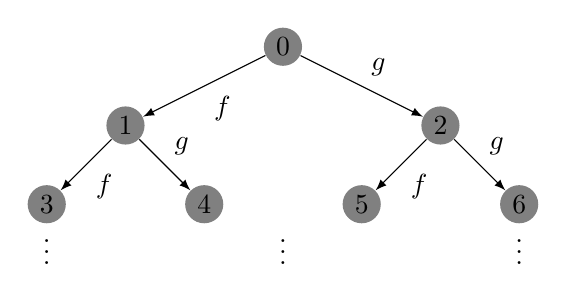
\begin{tikzpicture}
	\begin{pgfonlayer}{nodelayer}
		\node [style={filled_vertex}] (0) at (0, -0) {0};
		\node [style={filled_vertex}] (1) at (-2, -1) {1};
		\node [style={filled_vertex}] (2) at (2, -1) {2};
		\node [style={filled_vertex}] (3) at (-3, -2) {3};
		\node [style={filled_vertex}] (4) at (-1, -2) {4};
		\node [style={filled_vertex}] (5) at (1, -2) {5};
		\node [style={filled_vertex}] (6) at (3, -2) {6};
		\node [style=none] (7) at (0, -2.5) {$\vdots$};
		\node [style=none] (8) at (3, -2.5) {$\vdots$};
		\node [style=none] (9) at (-3, -2.5) {$\vdots$};
	\end{pgfonlayer}
	\begin{pgfonlayer}{edgelayer}
		\draw [style=transition] (0) to node[auto]{$f$} (1);
		\draw [style=transition] (1) to node[auto]{$f$} (3);
		\draw [style=transition] (1) to node[auto]{$g$} (4);
		\draw [style=transition] (0) to node[auto]{$g$} (2);
		\draw [style=transition] (2) to node[auto]{$f$} (5);
		\draw [style=transition] (2) to node[auto]{$g$} (6);
	\end{pgfonlayer}
\end{tikzpicture}


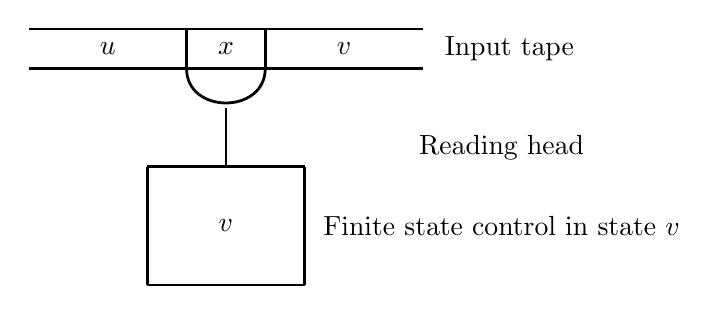
\begin{tikzpicture}
	\begin{pgfonlayer}{nodelayer}
		\node [style=none] (0) at (-1, -0) {};
		\node [style=none] (1) at (0, -0) {};
		\node [style=none] (2) at (-1, -0.5) {};
		\node [style=none] (3) at (0, -0.5) {};
		\node [style=none] (4) at (-3, -0) {};
		\node [style=none] (5) at (-3, -0.5) {};
		\node [style=none] (6) at (2, -0) {};
		\node [style=none] (7) at (2, -0.5) {};
		\node [style=none] (8) at (-1, -0.5) {};
		\node [style=none] (9) at (0, -0.5) {};
		\node [style=none] (10) at (-1.5, -1.75) {};
		\node [style=none] (11) at (0.5, -1.75) {};
		\node [style=none] (12) at (-1.5, -3.25) {};
		\node [style=none] (13) at (0.5, -3.25) {};
		\node [style=none] (14) at (-0.5, -1) {};
		\node [style=none] (15) at (-0.5, -1.75) {};
		\node [style=none] (16) at (-2, -0.25) {$u$};
		\node [style=none] (17) at (-0.5, -0.25) {$x$};
		\node [style=none] (18) at (1, -0.25) {$v$};
		\node [style=none] (19) at (-0.5, -2.5) {$v$};
		\node [style=none] (20) at (3.1, -0.25) {Input tape};
		\node [style=none] (21) at (3, -1.5) {Reading head};
		\node [style=none] (22) at (3, -2.5) {Finite state control in state $v$};
	\end{pgfonlayer}
	\begin{pgfonlayer}{edgelayer}
		\draw [style=simple] (4.center) to (0.center);
		\draw [style=simple] (0.center) to (1.center);
		\draw [style=simple] (1.center) to (6.center);
		\draw [style=simple] (5.center) to (2.center);
		\draw [style=simple] (2.center) to (3.center);
		\draw [style=simple] (3.center) to (7.center);
		\draw [style=simple] (0.center) to (2.center);
		\draw [style=simple] (1.center) to (3.center);
		\draw [style=simple, bend right=90, looseness=1.50] (8.center) to (9.center);
		\draw [style=simple] (8.center) to (9.center);
		\draw [style=simple] (10.center) to (11.center);
		\draw [style=simple] (11.center) to (13.center);
		\draw [style=simple] (13.center) to (12.center);
		\draw [style=simple] (12.center) to (10.center);
		\draw [style=simple] (14.center) to (15.center);
	\end{pgfonlayer}
\end{tikzpicture}

\begin{texexample}{Square Roots}{ex:sqrt10}
$\sqrt{2}^{{\sqrt{2}}^{\sqrt{2}}} = $
\begin{luacode}
local result=math.sqrt(2)^(math.sqrt(2))^(math.sqrt(2))
tex.print(result)
\end{luacode}
\end{texexample}


